\documentclass[12pt]{article}
\usepackage[left=1.2in,right=1.2in,top=1.2in,bottom=1.2in]{geometry}
\usepackage{lipsum}
\usepackage[hidelinks]{hyperref}
\urlstyle{same}
\usepackage{multicol}
\usepackage{footmisc}
  
\usepackage{mathtools}
\usepackage{amsmath}
\usepackage{amsfonts}
\usepackage{amssymb}
\usepackage{gensymb}

\usepackage[utf8]{inputenc}

% For nicely formatted header (choose what the left, right and center headers and footers say) (\thepage gives the page number, \leftmark gives section title and \rightmark gives the subsection title)
\usepackage{fancyhdr}
\pagestyle{fancy}
\lhead{}
\chead{}
\rhead{Daniel Widdowson, 201459067}
\lfoot{}
\cfoot{\thepage}
\rfoot{}
\renewcommand{\headrulewidth}{0.4pt}
\renewcommand{\footrulewidth}{0.4pt}
\renewcommand{\thefootnote}{[\arabic{footnote}]}

\begin{document}

\null

   \begin{center}
      \Large\textbf{Project Specification and Proposed Design}\\
      \large{Daniel Widdowson, 201459067}
   \end{center}

\null

\null

\section{Summary}

The aim of this project is to investigate a specific challenge in computational geometry, the motivation for which lies in crystallography. The project will be carried out with a general eye towards developing new methods for visualisation, analysis and prediction of crystal structures. 

\section{Motivation}

Since the advent of computers, \emph{crystal structure prediction} (CSP) has been an active area of research aiming to discover new potential crystal structures (\emph{metastable polymorphs}). The methods tend to involve exploring the space of all potential crystals trying to minimise an energy function, as stable structures are low-energy. 

Standard CSP algorithms suffer from \emph{over-prediction}; they output far too many crystals at local minima of the energy function. These minima are usually hinting at a small collection of distinct stable crystals each separated by barriers of high energy, but modern CSP methods waste time considering nearly identical crystals. Indeed, if one good candidate for a metastable polymorph is found, then a slight perturbation of it is likely to minimize the energy function quite well. 

So naturally, some way of identifying whether two crystals are `close' or properly distinct in this sense would be useful. An ideal goal is some function from the space of crystals to some numeric space which is 1) \emph{continuous} (\emph{stable-under-noise}), 2) \emph{invariant} under isometries (isometric crystals are identical under the function), and 3) complete under isometries (if two crystals coincide under the function then they are isometric). 

\null

This problem sat in the overlap between crystallography and computer science is part of the the domain known as \emph{computational geometry}. In short, the problem could be referred to as \emph{a continuous, isometric classification of crystals}.

\section{Background}

\subsection{Crystal/periodic set, lattice, unit cell, motif}

\textsc{non-technical.} A \emph{periodic crystal} in 3D is defined by a finite \emph{motif} of atoms or ions in a \emph{unit cell}, which is translated periodically along the edges of the cell ad infinitum. The motif is a finite collection of positions of atoms, and the unit cell is a parallelepiped (usually specified by three lengths and three angles). Positions of atoms in the motif are usually given with respect to the unit cell, i.e. the position `relative' to the unit cell, as three numbers between 0 and 1 indicating how far along each axis of the cell the atom is positioned. Here is an example of a unit cell and motif consisting of one molecule (rendered in Mercury):

\begin{center}
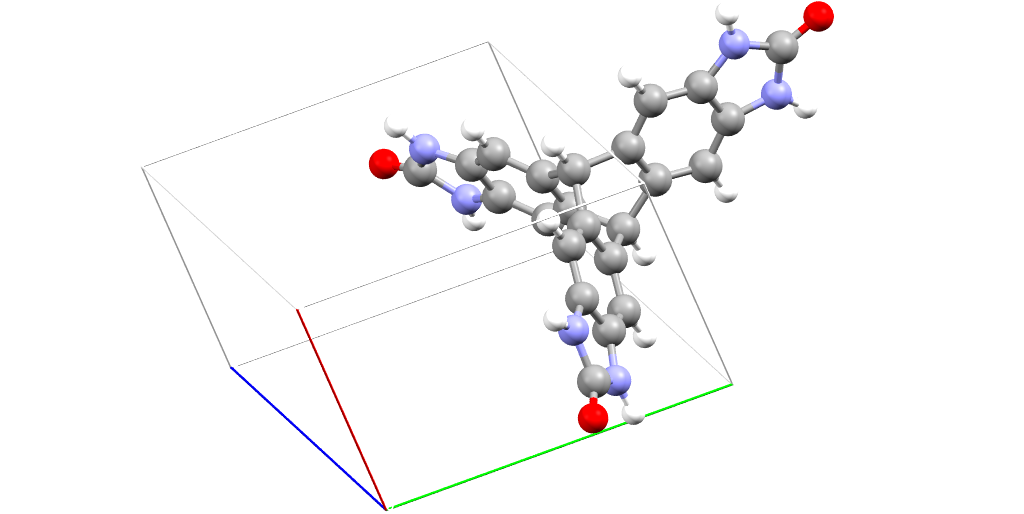
\includegraphics[scale=0.4]{job_03351.png}
\end{center}

To obtain the whole periodic crystal, the cell and motif are repeated along all three directions (theoretically infinitely). Note that information such as atomic bonds are not part of the mathematical model of a crystal, hence they may or may not be included when specifying a crystal; instead they might be inferred by inter-atomic distances. This and other (potentially) relevant information such as atomic types or charges can be worked into the mathematical model if needed (see the technical section for more detail). 

\null

\noindent\textsc{technical.} Given a basis $\{v_i\}_{i=1}^n$ of $\mathbb{R}^n$, we define a  \emph{lattice} $\Lambda$ and a \emph{unit cell} $U$ as
\[
\Lambda = \left\{\sum_{i=1}^n \lambda_i v_i \,\mid \, \lambda_i\in\mathbb{Z}\right\} \qquad\qquad
U = \left\{\sum_{i=1}^n \mu_iv_i \mid \mu_i\in [0,1) \right\}
\]
and a \emph{motif} $M$ is defined as some finite collection of points in $U$. Then a \emph{crystal} or \emph{periodic set} $S$ is the natural sum (\emph{Minkowski sum}) of $\Lambda$ and $M$, 
\[
S = \Lambda + M = \{u+v\mid u\in \Lambda, v\in M\}
\]
\emph{Note.} This definition extends to $\mathbb{R}^n$, as might other statements regarding periodic sets. However when it comes to application we're only concerned with $\mathbb{R}^3$, so at some point it might be reasonable to drop the generality of working in $\mathbb{R}^n$ in favour of the concreteness/simplicity of working in $\mathbb{R}^3$ alone.

\noindent\emph{Note. }If necessary, we might want to include information like atomic types alongside each point in the motif. This can be done \emph{combinatorially}, for example by defining $M$ as a set of ordered pairs (position, atomic number). It's important to remember to only do this where it's explicitly needed, otherwise it'll likely serve to obfuscate rather than clarify or add anything relevant, especially when it comes to analyzing crystals purely geometrically.

\subsection{Invariants}

The concept of an \emph{invariant} is near universal in mathematics. In general, \emph{invariance} can be summarized as `stability under change', or, the property of remaining unchanged regardless of certain transformations. A simple example would be the area of a surface with respect to translation or rotation; the area does not change under these transformations and thus area is an invariant of surfaces with respect to rotations and translations. 

Note: The idea of invariants reaches much deeper than this though, for example the exponential function $e^x$ is an invariant of differentiation, and the bell curve (Gaussian function) is invariant under the Fourier transform. Indeed a mathematician might argue that the prevalence of $e^x$ and the bell curve is down to them being invariants of natural transformations. 

 A major CSP problem is to classify crystals in a way that is \emph{invariant under isometry}, that is, finding a function which classifies crystals such that two isometric crystals are identical under the function. The project will not tackle this problem directly, but will investigate some specific ideas relating to the problem.

\section{Recent discoveries}

Recent research \cite{MoscaKurlin} points towards a potentially significant measure regarding periodic crystals. Let $S = \Lambda + M$ denote a periodic set with lattice $\Lambda$ and motif $M$ with $m$ points. Given natural $k\geq 1$, define the \emph{pointwise distribution of distances} PDD$(S;k)$ to be a matrix such that PDD$(S;k)_{ij}$ is the distance from the $i$th point in the motif to its $j$th nearest neighbour. In other words, PDD$(S;k)$ has one row for each point in the motif, and a row consists of distances from that particular point to its nearest neighbours in the motif. 

Such a matrix can be ordered sensibly, and then reduced by collapsing identical rows and keeping their \emph{weight}. The weight of a row in a PDD is the number of times it appears in the matrix divided by $m$. Then we define the \emph{average minimum distance} AMD$_k$ as a weighted average of the last column of the PDD. 

\cite{MoscaKurlin} proves isometric invariance of the AMD, and its stability under perturbations of the periodic set. It was found that for small $k$, AMD$_k$ grows in a way that is not smooth, and AMD$_k$ is not all that different between crystals. However as $k$ grows, smooth asymptotic behaviour emerges and AMD$_k$ diverges for different crystals. The smooth curves are roughly log-like, though it was found to not actually exhibit logarithmic behaviour. 

A specific sub-goal of this project is to properly identify the `log-like' behaviour exhibited by AMD$_k$ and to pin down a parameter which neatly describes AMD$_k$ given a crystal. This should lead to further investigation of this measure of similarity.

\section{Software}

The software required for this project will need to be capable of visualisation and analysis of crystals read in from .cif files. Well-known and widely used software such as Mercury is built for this purpose, so in some cases it will not be necessary to design and implement code to do this. However Mercury is a general-purpose program and this project has a relatively specific direction, so it will be necessary to design some algorithms for our specific purposes.

Explicit visualisation of data used is a massively useful tool, being an aid to common-sense heuristics (e.g. if one is manipulating atomic positions in a crystal, displaying the crystal is likely to provide immediate evidence whether the algorithm working as intended or not). In our case, this would involve rendering atoms' positions in space onto the screen, as well as elements such as the unit cell, atomic bonds, etc. Mercury is good at reading and displaying the contents of .cif files, however if additional elements need to be added to the display, this will need to be done using software for visualisation written for this project.

With regards to analysis, all but the most common methods of analysis will have to be implemented; this is likely to be a large portion of the code written.

The visualisation and analysis parts of the software will be kept logically separated, but will be able to `work together' (i.e. be very compatible).

\section{Data Usage}

The data used in this project will be entirely synthetic and will not involve human participants. The data required will involve \emph{crystallographic information files} (.cif) containing data  specifying periodic crystals. These files will be sourced either from the supervisor(s) of this project or possibly from publicly available databases if needed.

\begin{thebibliography}{9}
\bibitem{MoscaKurlin} 
M. Mosca and V. Kurlin. \emph{Algorithmic challenges of computational geometry motivated by applications in crystallography}. 2020.
\end{thebibliography}

 
\end{document}